\chapter{Main Program}
\label{main-program}

The general idea is to build an UI with three main divisions: Home (with device
selection), midi selection and signal-to-MIDI connections, Plot (with the signal
visualization) and Options (with the algorithm tuning options, as well as virtual
MIDI creation).\\
When a device is selected it's signals will go through a simple process, as in \autoref{signals-flow-diagram}.
\begin{figure}[htb]
	\caption{Signals Flow Diagram}
  \label{signals-flow-diagram}
	\begin{center}
    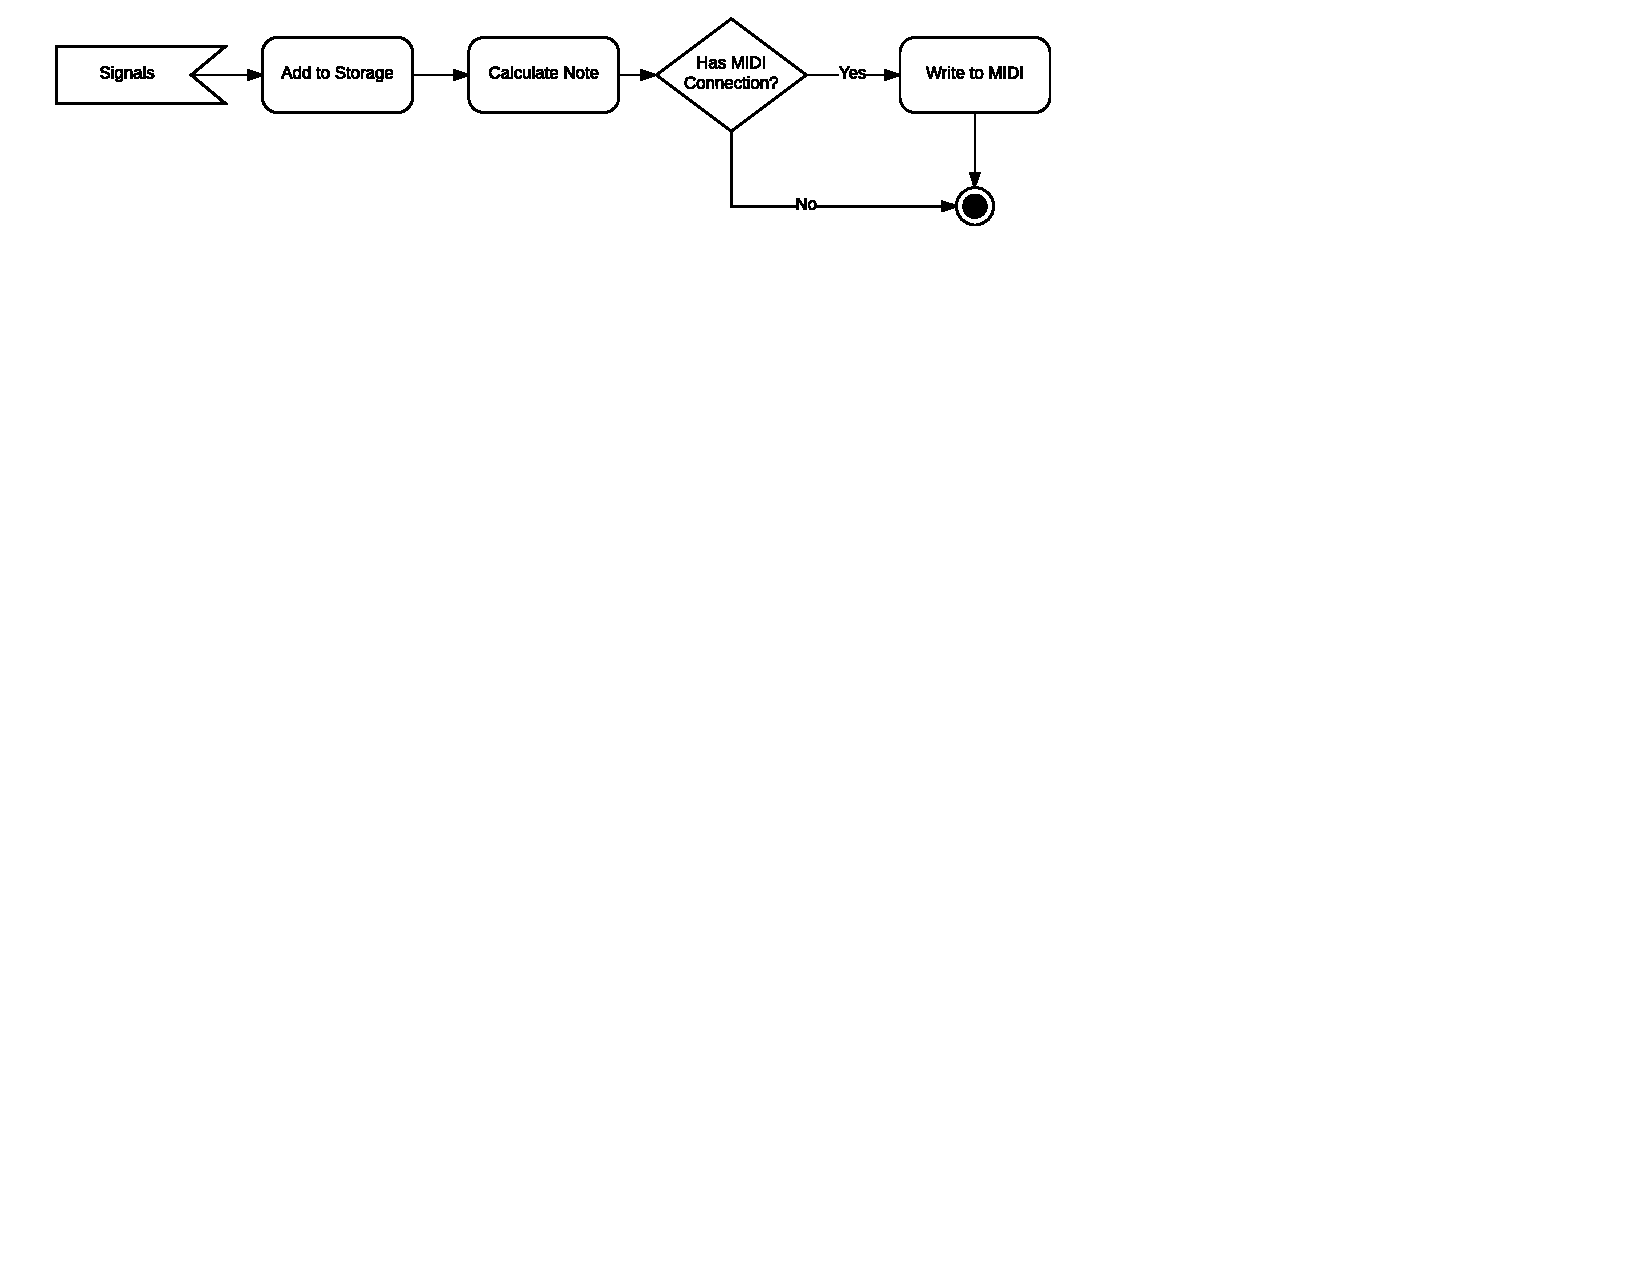
\includegraphics[scale=0.9]{images/signals-flow-diagram.pdf}
	\end{center}
  \legend{Source: made by authors}
\end{figure}

\section{GUI}

\subsection{Home}
The home page has three horizontally divided sections: Device and signals, MIDI selection
and list, and  finally connections, as in \autoref{home-page}. \\
The first is used to open the device (there can be only one used at a time). When it
is open a list of signals will be displayed (six of them, named as each guitar note).
Each signal can be selected so it can be connected to a MIDI device.\\
The second is to open any given number of existing MIDI devices, which will be listed
bellow (can be also closed). The listed devices can also be selected, but only one at a time. \\
The final section is used to establish the connections, given the selected signals
and MIDI, the connections are showed in the box bellow and can be deleted.
\begin{figure}[htb]
	\caption{Home Page}
  \label{home-page}
	\begin{center}
    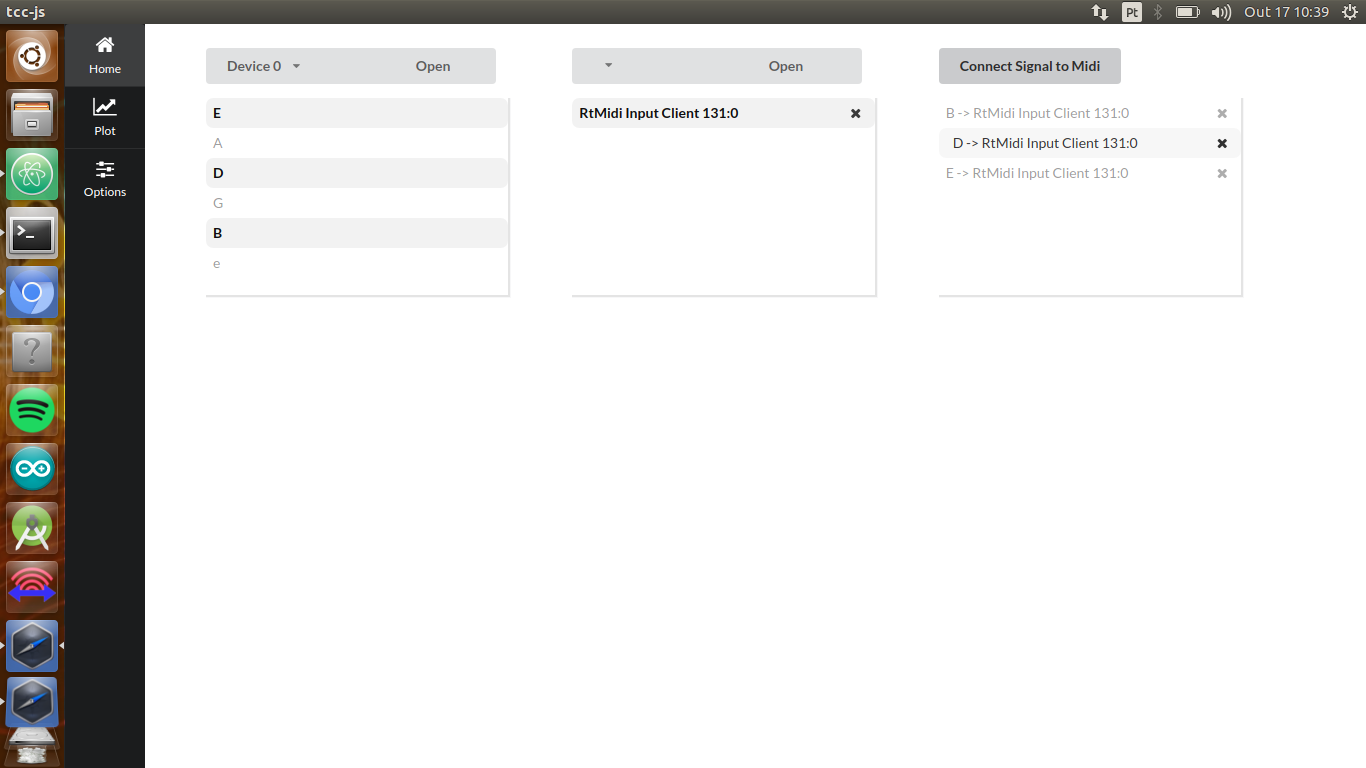
\includegraphics[width=0.7\paperwidth]{images/snapshots/home.png}
	\end{center}
  \legend{Source: authors}
\end{figure}

\subsection{Plot}
The Plot page is a simply a react-plotter \cite{react-plotter} component with a few
visual controls, being: a dropdown to select which signal is being displayed,
a checkbox to enable trigger, a slider to control the time
range and another slider to control the trigger value. The full page is as in \autoref{plot-page}.
It was chosen to show only one plot at a time so it's size is bigger, easier to see.
This also makes the program a little more performant.
\begin{figure}[htb]
	\caption{Plot Page}
  \label{plot-page}
	\begin{center}
    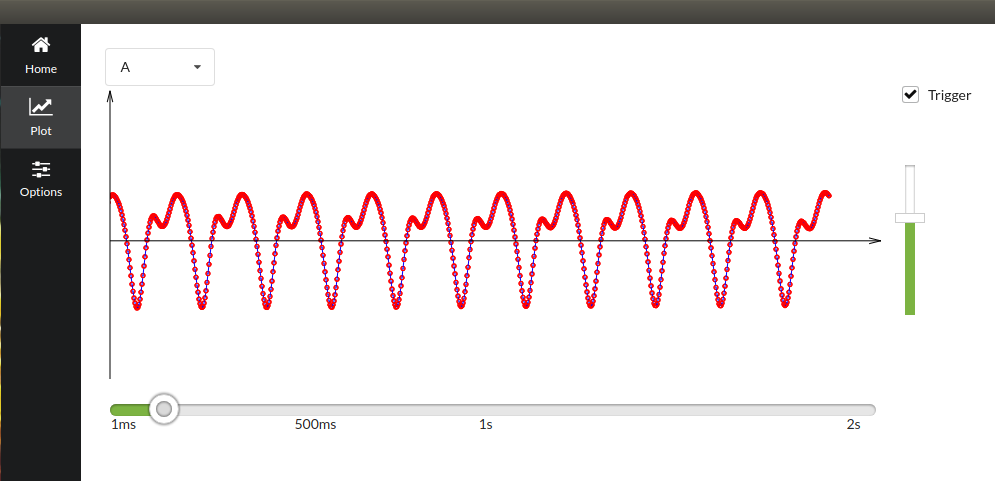
\includegraphics[width=0.7\paperwidth]{images/snapshots/plot-trigger-A.png}
	\end{center}
  \legend{Source: authors}
\end{figure}

\subsection{Options Page}
% TODO
